\documentclass[12pt, a4paper]{article}
\usepackage[utf8]{vietnam}
\usepackage[left = 1cm, right = 1cm, top = 2cm, bottom = 2cm]{geometry}
\usepackage{indentfirst}
\setlength{\parindent}{1cm}
\usepackage{tikz}
\usepackage{xcolor}
\makeatletter\newcommand{\Letter}[1]{\@Alph{#1}}\makeatother
\usepackage{calc}
\usetikzlibrary{patterns} 

\usepackage{wrapfig}
\usepackage{graphicx}
\usepackage{caption}

\begin{document}
	
	\tikzset{mystyle/.style={draw = blue,  thick, ->}}
	% picture 1
	\begin{flushleft}
		
		\begin{tikzpicture}
			% create a lưới to paint the way easy
			% \draw [help lines] (-5,-5) grid (5,5);
			
			% Create node
			\node [below left] at (0,0) {0};
			\node [below right] at (1.5,0) {$59$};
			\node[below left] at (0,3) {$61$};
			\node[below left] at (0,4.26) {120};
			\node[below right] at (0.4,4.26) {A};
			\node[below left] at (4.26,0) {120};
			\node[below left] at (4.26,0) {120};
			\node[above] at (4.26,0) {B};
			\node[above] at (4,2.3) {$x^*=(59,16)$};
			
			
			
			
			
			% draw cung tròn
			\fill (0,0) circle (2pt);
			\draw[mystyle,very thick,->] (-0.5,0)--(5,0) node [right] {$x_1$};
			\draw[mystyle, very thick,->] (0,-0.5)--(0,5) node [above] {$x_2$};
			\draw[dashed] (0,0) circle (0.6cm);
			\draw[dashed]  (1.5,0) arc (0:100:1.5);
			\draw[dashed]  (2,0) arc (0:100:2);
			\draw[dashed]  (2.5,0) arc (0:100:2.5);
			\draw[dashed]  (3,0) arc (0:100:3);
			\draw (0,4.26)--(4.26,0);
			
			
			\draw[very thick,->] (3,3.5)--(2.3,2.7) node [pos = -0.3] {$x_1+x_2=120$};
			\draw[very thick,->] (-1,3)--(-0.5,3) node [pos = -1.7] {$f = f_{min}$}; % sửa đoạn này
			\draw[dashed,very thick,->] (-1,1)--(0,0.6) node [pos = -0.7] {$f = const$};
			\draw[dashed,very thick,->] (-1,1)--(0,1.5);
			\draw[dashed,very thick,->] (-1,1)--(0,2);
			\draw[dashed,very thick,->] (-1,1)--(0,2.5);
			\draw[dashed] (2.1,0)--(2.1,2.1)--(0,2.1);
			
			
			
			
		\end{tikzpicture}
		
		
	\end{flushleft}
	
	\begin{flushright}
		\begin{figure}
			\centering
			\includegraphics{photo/draw2.png}
			\label{fig:my_label}
		\end{figure}
	\end{flushright}
	
	%picture 3
	\begin{center}
		
		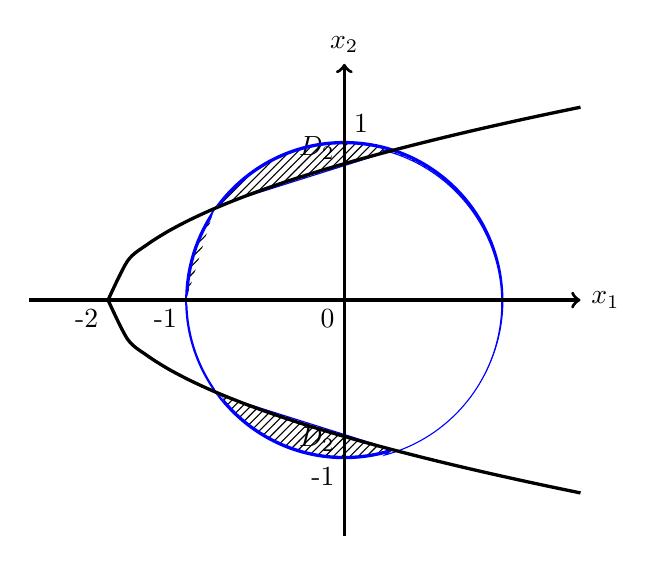
\begin{tikzpicture}
			% \draw [help lines] (-5,-5) grid (5,5);
			% node point
			
			\node[below left] at (-3,0) {-2};
			\node[below left] at (-2,0) {-1};
			\node[below left] at (2,0) {1};
			\node[below left] at (0,-2) {-1};
			\node[above right] at (0,2) {1};
			\node[below left] at (0,2.2) {$D_2$};
			\node[below left] at (0,-1.5) {$D_2$};
			
			
			% draw
			
			\fill[draw =blue, pattern=north east lines,smooth , very thick] (0,0) circle (2cm);
			
			
			
			
			% vẽ hàm số
			
			
			\draw[fill = white, draw = blue] (2,0) arc (1:75:2) -- (0.612,1.9)--(-1.61,1.2)
			(2,0) arc (1:-75:2) -- (0.612,-1.9)--(-1.61,-1.2)
			(-2,0) arc (-180:-140:2);
			\draw[fill = white, draw = white] (-1.61,1.2)--(2,0)--(-1.61,-1.2)--(-2,0)--(-1.66,1.1)--(-1.60,1.2);
			
			
			\draw[domain = -3:3, smooth, very thick] plot (\x ,{((\x)+3)^0.5})plot (\x ,{-((\x)+3)^0.5});
			
			
			
			\node [below left] at (0,0) {0};
			\draw[very thick, ->] (0,-3)--(0,3) node [above] {$x_2$};
			\draw[very thick, ->] (-4,0)--(3,0) node [right] {$x_1$};
			
			
		\end{tikzpicture}
		
		
	\end{center}
	
	
	
	
	
	% photo 4
	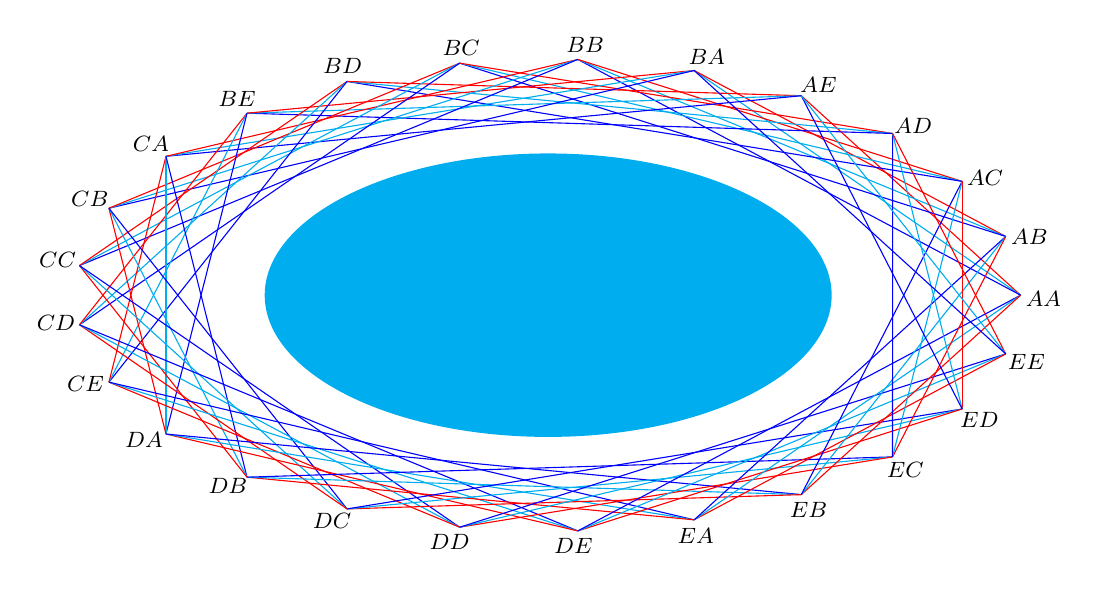
\begin{tikzpicture}[declare function={a=6;b=3;n=25;k=5;g=360/n;},font=\footnotesize]
		\fill[cyan] ellipse (.6*a and .6*b);
		\foreach \i[parse=true] in{0,...,(n-1)}{
			\pgfmathsetmacro{\m}{int(\i/k)+1}
			\pgfmathsetmacro{\p}{mod(\i,k)+1}
			\path (\i*g:a and b) node[shift={(g*\i-g:.3 and .2)}]{$\Letter{\m}\Letter{\p}$};
			\draw[red] (\i*g:a and b)--({g*(\i+4)}:a and b);
			\draw[cyan] (\i*g:a and b)--({g*(\i+5)}:a and b);
			\draw[blue] (\i*g:a and b)--({g*(\i+6)}:a and b);
		}
	\end{tikzpicture}
	
	
	
\end{document}